\documentclass[conference]{IEEEtran}

\usepackage[utf8]{inputenc}
\usepackage[T1]{fontenc}
\usepackage[spanish,es-tabla,es-nodecimaldot,es-noshorthands]{babel}
\usepackage{amsmath,amssymb}
\usepackage{graphicx}
\usepackage{booktabs}
\usepackage{listings}
\usepackage{framed}
\usepackage{xcolor}
\usepackage{cite}
\usepackage{url}

% Marca en rojo para lo que falta completar (debe desaparecer en la versión final)
\newcommand{\pendiente}[1]{\textcolor{red}{\textbf{[PENDIENTE: #1]}}}

\lstset{
  language=Matlab,
  basicstyle=\ttfamily\scriptsize,
  keywordstyle=\color{blue},
  commentstyle=\color{green!50!black},
  stringstyle=\color{purple},
  breaklines=true,
  frame=single,
  numbers=left,
  numberstyle=\tiny,
  columns=fullflexible,
  showstringspaces=false
}

\begin{document}

\title{Diseño de controlador y observador\\ Tarea Examen Control Automático}

\author{
\IEEEauthorblockA{Escuela de Ingeniería Electrónica\\
Tecnológico de Costa Rica\\
EL-5408 Control Automático\\
II Semestre 2026\\
Esquivel Salazar Greivin (2023102615), López Méndez Abner (2022273075), Segura Chinchilla Jordi (2022240646)\\
gresquivel@estudiantec.cr, ablopez@estudiantec.cr, jorsegura@estudiantec.cr}
}

\maketitle

\begin{abstract}
En este trabajo se diseña un sistema de control para el convertidor DC-DC del problema 36 del capítulo 12 del libro de Nise. El sistema está formado por un controlador por realimentación de estados con acción integral, que elimina el error en estado estacionario, y por un observador de estados diez veces más rápido que el controlador. Las especificaciones de diseño son un sobreimpulso del 20\,\% y un tiempo de establecimiento de 0.5\,s. El diseño se solicitó primero a una inteligencia artificial (IA) gratuita mediante un prompt estructurado, y su respuesta se comparó con los cálculos propios, realizados en un Live Script de MATLAB. Finalmente, el sistema completo se implementó en Simulink con condiciones iniciales distintas en la planta y en el observador. Se obtuvo un sobreimpulso de 19.46\,\%, un tiempo de establecimiento de 0.487\,s, error en estado estacionario nulo y un error de estimación que se anula en menos de 0.1\,s. \pendiente{Una frase con el veredicto sobre la respuesta de la IA.}
\end{abstract}

\begin{IEEEkeywords}
Realimentación de estados, observador, control integral, convertidor DC-DC, inteligencia artificial, Simulink.
\end{IEEEkeywords}

\section{Introducción}

La realimentación de estados permite ubicar todos los polos de lazo cerrado de un sistema, pero supone que todos los estados se pueden medir. En el convertidor estudiado solo se mide el voltaje del capacitor, por lo que la corriente del inductor se debe estimar con un observador. Además, la realimentación de estados por sí sola no garantiza que la salida siga a la referencia, así que se agrega un integrador del error para eliminar el error en estado estacionario \cite{nise}.

El objetivo del trabajo es diseñar estas tres partes (controlador, observador y corrección del error en estado estacionario) y se divide en tres etapas: (1)~obtener el diseño con una IA gratuita a partir de un prompt bien planteado, (2)~comprobar con un Live Script de MATLAB si el procedimiento de la IA es correcto y (3)~implementar el sistema en Simulink, demostrando que el observador converge aunque arranque con condiciones iniciales distintas a las de la planta.

\section{Modelo de la planta}

La planta es el convertidor DC-DC del problema 36 de \cite{nise}, con $L = 6$\,mH, $C = 1$\,mF, $R = 100\,\Omega$ y un ciclo de trabajo del 50\,\%. Sus ecuaciones de estado son
\begin{equation}
\begin{bmatrix} \dot{i}_L \\ \dot{u}_C \end{bmatrix} =
\begin{bmatrix} 0 & -83.33 \\ 500 & -10 \end{bmatrix}
\begin{bmatrix} i_L \\ u_C \end{bmatrix} +
\begin{bmatrix} 166.67 \\ 0 \end{bmatrix} E_s
\end{equation}
\begin{equation}
y = \begin{bmatrix} 0 & 1 \end{bmatrix} \begin{bmatrix} i_L \\ u_C \end{bmatrix}
\end{equation}
donde la salida es el voltaje del capacitor $u_C$. A estas matrices se les llama $A_z$, $B_z$ y $C_z$. La función de transferencia, obtenida con \texttt{ss2tf}, es
\begin{equation}
G(s) = \frac{U_C(s)}{E_s(s)} = \frac{83335}{s^2 + 10s + 41665}
\end{equation}

\section{Diseño}

\subsection{Polos del controlador}

Las especificaciones son las que plantea el propio problema~36 de \cite{nise}: 20\,\% de sobreimpulso y tiempo de establecimiento de 0.5\,s. El factor de amortiguamiento y la frecuencia natural son
\begin{equation}
\zeta = \frac{-\ln(0.20)}{\sqrt{\pi^2 + \ln^2(0.20)}} = 0.4560
\end{equation}
\begin{equation}
\omega_n = \frac{4}{\zeta T_s} = 17.546~\text{rad/s}
\end{equation}
con lo que la ecuación característica deseada del controlador es
\begin{equation}
s^2 + 16s + 307.855 = 0
\end{equation}
y sus polos son $s_{1,2} = -8 \pm j15.616$.

\subsection{Observador}

Primero se verificó que el sistema es observable. La matriz de observabilidad en las coordenadas originales es
\begin{equation}
O_z = \begin{bmatrix} C_z \\ C_z A_z \end{bmatrix} =
\begin{bmatrix} 0 & 1 \\ 500 & -10 \end{bmatrix}
\end{equation}
que tiene rango 2, por lo que el sistema es observable.

Para facilitar el cálculo de las ganancias, el sistema se escribió en forma canónica observable a partir de $G(s)$:
\begin{equation}
A_x = \begin{bmatrix} -10 & 1 \\ -41665 & 0 \end{bmatrix},\quad
B_x = \begin{bmatrix} 0 \\ 83335 \end{bmatrix},\quad
C_x = \begin{bmatrix} 1 & 0 \end{bmatrix}
\end{equation}
En esta forma, la ecuación característica del observador $\det(sI - (A_x - L_x C_x))$ queda directamente como
\begin{equation}
s^2 + (10 + l_1)s + (41665 + l_2) = 0
\end{equation}

Para que el observador sea diez veces más rápido que el controlador, sus polos se ubicaron en diez veces los polos del controlador, $s = -80 \pm j156.16$. Esto mantiene el mismo $\zeta$ y reduce diez veces el tiempo de establecimiento. La ecuación deseada del observador es
\begin{equation}
s^2 + 160s + 30785.5 = 0
\end{equation}
Igualando coeficientes se obtiene $l_1 = 150$ y $l_2 = -10880$.

Finalmente, la ganancia se transformó a las coordenadas originales con $L_z = P L_x$, donde
\begin{equation}
P = O_z^{-1} O_x = \begin{bmatrix} 0 & 0.002 \\ 1 & 0 \end{bmatrix},\quad
O_x = \begin{bmatrix} 1 & 0 \\ -10 & 1 \end{bmatrix}
\end{equation}
lo que da
\begin{equation}
L_z = \begin{bmatrix} -21.759 \\ 150 \end{bmatrix}
\end{equation}
Se comprobó que los valores propios de $A_z - L_z C_z$ son $-80 \pm j156.16$.

\subsection{Controlador con acción integral}

Antes de calcular $K$ se verificó que el sistema es controlable. La matriz de controlabilidad es
\begin{equation}
C_M = \begin{bmatrix} B_z & A_z B_z \end{bmatrix} =
\begin{bmatrix} 166.67 & 0 \\ 0 & 83335 \end{bmatrix}
\end{equation}
cuyo determinante es $1.389\times10^{7} \neq 0$. Tiene rango 2, por lo que existen ganancias que ubican los polos del lazo cerrado donde se desee.

Para eliminar el error en estado estacionario se agrega el estado del integrador $x_N$, que acumula el error entre la referencia $r$ y la salida \cite{nise}:
\begin{equation}
\dot{x}_N = r - C_z x, \qquad u = -Kx + k_e x_N
\end{equation}
con $K = [k_1\ \ k_2]$. El sistema aumentado queda
\begin{equation}
\begin{bmatrix} \dot{x} \\ \dot{x}_N \end{bmatrix} =
\begin{bmatrix} A_z - B_z K & B_z k_e \\ -C_z & 0 \end{bmatrix}
\begin{bmatrix} x \\ x_N \end{bmatrix} +
\begin{bmatrix} 0 \\ 1 \end{bmatrix} r
\end{equation}
y su ecuación característica, calculada en MATLAB, es
\begin{multline}
s^3 + (166.67k_1 + 10)s^2 \\
+ (1666.7k_1 + 83335k_2 + 41665)s + 83335k_e = 0
\end{multline}

Al agregar el integrador, el sistema pasa a ser de tercer orden, por lo que se necesita un tercer polo. Este se ubicó en $s = -80$, es decir, lo suficientemente alejado de los polos dominantes (diez veces su parte real) para que su efecto sobre la respuesta transitoria sea despreciable \cite{nise}. La ecuación deseada es entonces
\begin{multline}
(s^2 + 16s + 307.855)(s + 80) = \\
s^3 + 96s^2 + 1587.85s + 24628.4
\end{multline}
Igualando coeficientes se obtienen las ganancias
\begin{equation}
k_1 = 0.51599,\quad k_2 = -0.49124,\quad k_e = 0.29553
\end{equation}

\subsection{Sistema completo}

En el sistema completo el controlador usa los estados estimados $\hat{x}$ en lugar de los reales, y el observador está dado por
\begin{equation}
\dot{\hat{x}} = A_z \hat{x} + B_z u + L_z (y - C_z \hat{x})
\end{equation}
con $u = -K\hat{x} + k_e x_N$. Los valores propios del sistema completo (planta, integrador y observador) son $-8 \pm j15.616$, $-80$ y $-80 \pm j156.16$, es decir, los polos del controlador con integrador más los del observador. Esto concuerda con el principio de separación: el observador no modifica los polos que se diseñaron para el controlador.

Conviene precisar en qué sentido el observador es diez veces más rápido. La comparación se hace contra los polos dominantes, que son los que fijan el desempeño especificado \cite{nise}. El tercer polo, en $-80$, tiene la misma parte real que los polos del observador, pero su efecto sobre la respuesta es pequeño, como lo confirma que el sobreimpulso obtenido (19.46\,\%) sea casi el de un sistema de segundo orden puro.

\section{Diseño mediante inteligencia artificial}

\subsection{Herramienta y prompt}
Se utilizó \pendiente{herramienta, plan gratuito, modelo y fecha}. El prompt se redactó para que la IA resolviera el problema completo sin ambigüedades: incluye las matrices del modelo, las especificaciones, la estructura del control integral con sus signos, el criterio para el tercer polo, la definición de ``diez veces más rápido'' y el orden en que debe presentar los resultados. No incluye los resultados propios, para que la IA tuviera que resolver el problema por su cuenta. El texto exacto es el siguiente:

\begin{framed}
\small
\noindent Actúa como un profesor de Control Automático. Resuelve paso a paso el siguiente problema de diseño en espacio de estados, mostrando todas las ecuaciones intermedias y los resultados numéricos con al menos 4 cifras significativas.

\smallskip\noindent PLANTA (Nise, Control Systems Engineering, 7.ª ed., capítulo 12, problema 36)\\
Convertidor DC-DC tipo boost (modelo promediado) con L = 6 mH, C = 1 mF, R = 100 $\Omega$ y ciclo de trabajo d = 0.5. Estados x = [i\_L; u\_C] (corriente del inductor en A y voltaje del capacitor en V), entrada u = E\_s (V) y salida y = u\_C (V):

\smallskip\noindent A = [0 \ $-$83.33; 500 \ $-$10], \ B = [166.67; 0], \ C = [0 \ 1], \ D = 0

\smallskip\noindent Usa exactamente estas matrices (no recalcules los coeficientes a partir de L, C y R).

\smallskip\noindent REQUISITOS DE DISEÑO\\
1. Desempeño del controlador: 20 \% de sobreimpulso y tiempo de asentamiento de 0.5 s (criterio del 2 \%, Ts = 4/($\zeta\cdot\omega$n)).\\
2. Error de estado estacionario cero ante una entrada escalón, usando control integral con esta estructura: dx\_N/dt = r $-$ y, \ u = $-$K$\cdot$x + Ke$\cdot$x\_N, \ con K = [k1 \ k2].\\
3. Ubica el tercer polo del sistema aumentado 10 veces más a la izquierda que la parte real de los polos dominantes.\\
4. Observador de estado completo (Luenberger): dx\_est/dt = A$\cdot$x\_est + B$\cdot$u + L$\cdot$(y $-$ C$\cdot$x\_est), con L = [l1; l2]. El observador debe ser 10 veces más rápido que el controlador: sus dos polos deben ser los polos dominantes del controlador multiplicados por 10 (mismo $\zeta$, $\omega$n 10 veces mayor).\\
5. Haz el diseño directamente en las coordenadas originales (sin pasar a la forma de variables de fase), igualando el polinomio característico con el polinomio deseado.

\smallskip\noindent ENTREGA LOS RESULTADOS EN ESTE ORDEN\\
a) Polos de lazo abierto, $\zeta$, $\omega$n y función de transferencia U\_C(s)/E\_s(s).\\
b) Matrices de controlabilidad y observabilidad, sus determinantes y la conclusión.\\
c) $\zeta$, $\omega$n, $\omega$d, polos dominantes deseados, tercer polo y polinomio deseado de tercer orden.\\
d) Matriz del sistema aumentado en lazo cerrado, su polinomio característico en función de k1, k2 y Ke, el sistema de ecuaciones y los valores de K y Ke.\\
e) Polos deseados del observador, polinomio característico de (A $-$ L$\cdot$C) en función de l1 y l2, y los valores de L.\\
f) Ecuaciones del sistema completo controlador-observador-integrador (5 estados) y, usando el principio de separación, cuáles son sus 5 polos.\\
g) Verificación: sustituye tus ganancias y comprueba que los valores propios de las matrices de lazo cerrado coinciden con los deseados.\\
h) Una tabla resumen final con: polos dominantes, tercer polo, K, Ke, polos del observador y L.

\smallskip\noindent No uses MATLAB ni otro software para obtener los resultados: muestra el procedimiento analítico. Si haces alguna suposición, indícala explícitamente.
\end{framed}

La respuesta íntegra de la IA se incluye en el Apéndice~\ref{ap:ia}.

\subsection{Dificultades}
\pendiente{Resumen breve: número de intentos, qué se ajustó en el prompt y qué errores cometió la IA, si los hubo.}

\section{Implementación en Simulink}

El sistema se implementó en Simulink (Fig.~\ref{fig:simulink}). La planta se representa con su función de transferencia y el observador se construye con bloques de ganancia ($A_z$, $B_z$, $C_z$ y $L_z$), un sumador y un integrador vectorial. El controlador toma los estados estimados, los multiplica por $-K$ y les suma la acción integral $k_e x_N$.

Como la planta es un bloque de función de transferencia, la corriente real del inductor no está disponible en Simulink; por eso la comparación entre $i_L$ real y estimada se hizo con \texttt{lsim} en MATLAB, con las mismas condiciones iniciales. Todos los valores numéricos están escritos directamente en los bloques, por lo que el modelo se puede ejecutar sin correr antes ningún script. La planta arranca con condiciones iniciales nulas y el observador con $\hat{x}(0) = [0.5\ \ 1]^T$, es decir, $\hat{i}_L(0) = 0.5$\,A y $\hat{u}_C(0) = 1$\,V. La referencia es un escalón unitario aplicado en $t = 1$\,s, de modo que durante el primer segundo se puede observar la convergencia del observador y después la respuesta al escalón. La simulación dura 2\,s con un paso máximo de 1\,ms.

\begin{figure*}[!t]
\centering
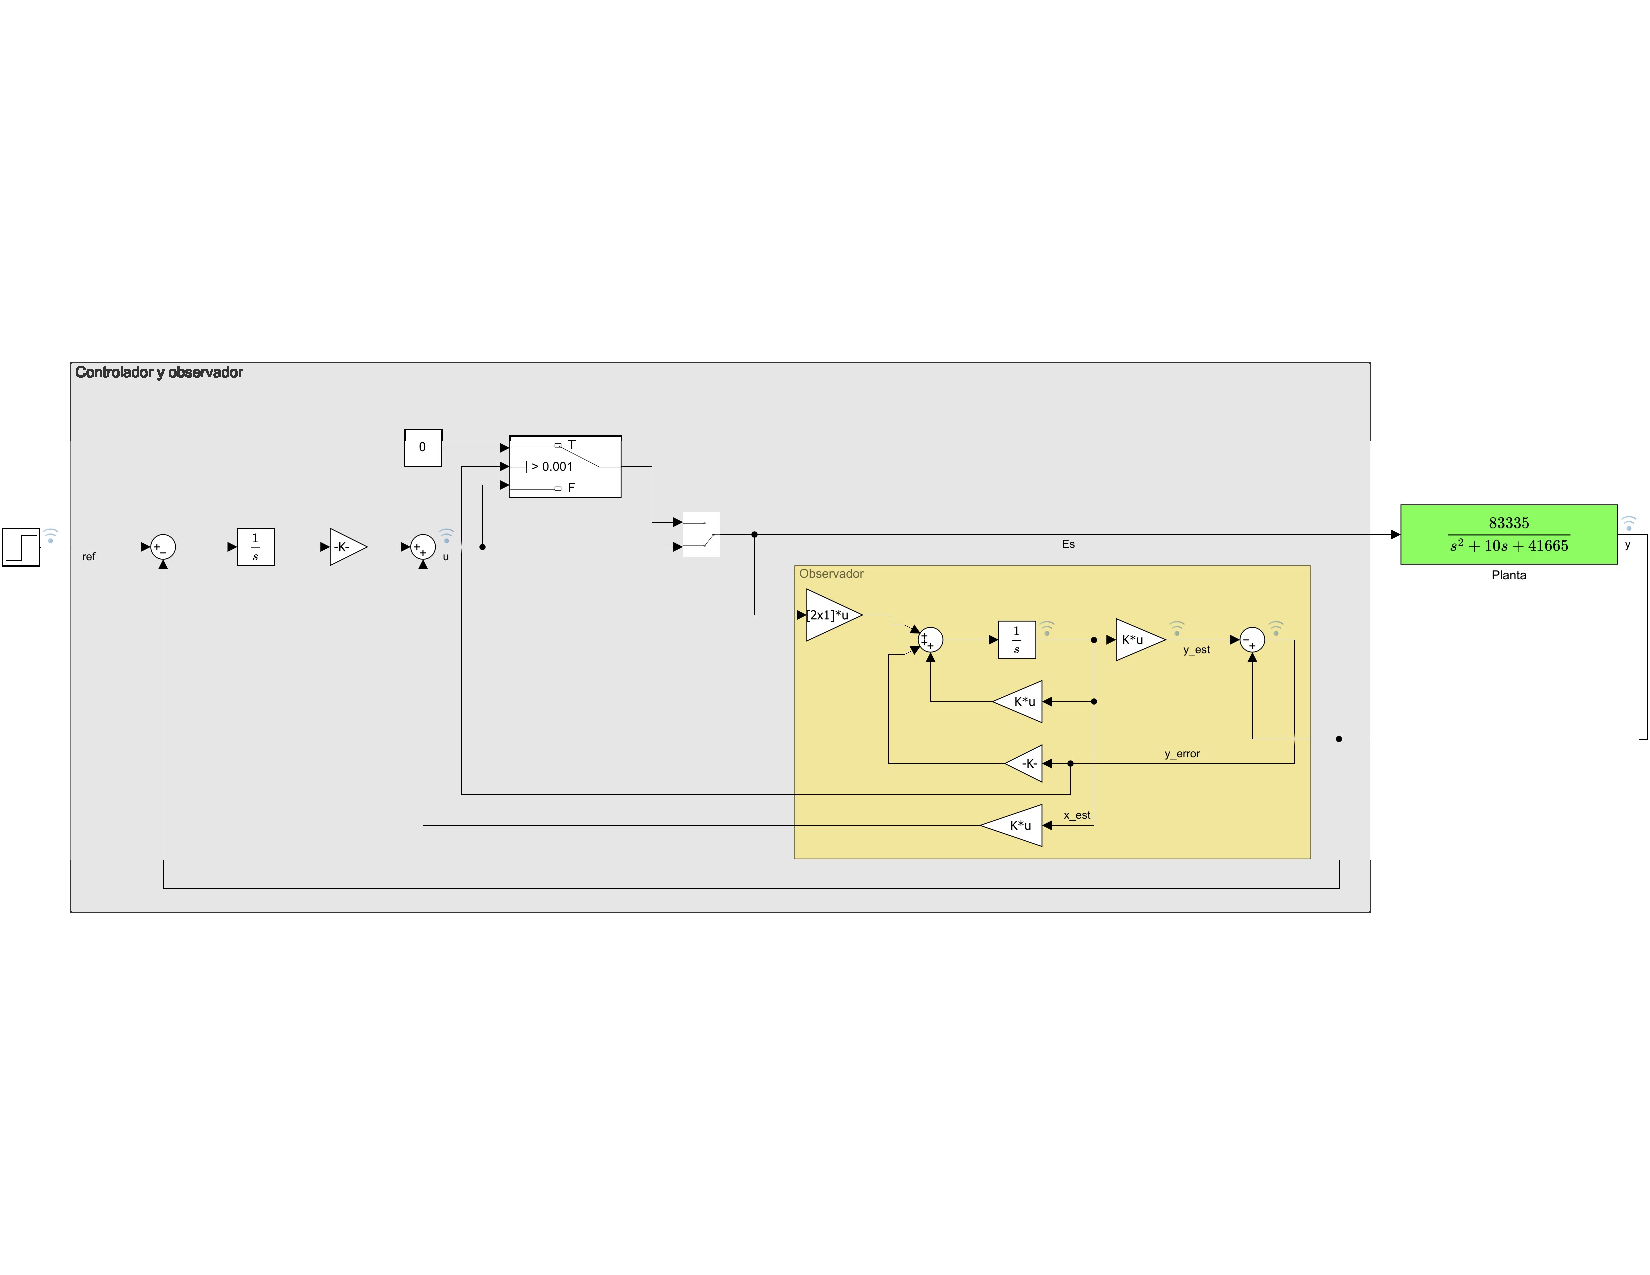
\includegraphics[width=0.95\textwidth,trim=20 150 20 150,clip]{Diagrama_simulink.pdf}
\caption{Modelo en Simulink del sistema controlador-observador-integrador.}
\label{fig:simulink}
\end{figure*}

\section{Resultados}

\subsection{Resultados numéricos}

Los resultados de los cálculos del Live Script (Apéndice~\ref{ap:livescript}) se resumen en la Tabla~\ref{tab:resultados}. La respuesta al escalón del sistema con integrador tiene un sobreimpulso de 19.46\,\% y un tiempo de establecimiento de 0.487\,s, por lo que se cumplen ambas especificaciones. El sobreimpulso queda un poco por debajo del 20\,\% porque el tercer polo, aunque está lejos, amortigua ligeramente la respuesta. La ganancia en DC del sistema completo es 1, lo que confirma que el error en estado estacionario es cero.

\begin{table}[!t]
\centering
\caption{Resultados del diseño}
\label{tab:resultados}
\begin{tabular}{@{}ll@{}}
\toprule
Parámetro & Valor \\
\midrule
Polos del controlador & $-8 \pm j15.616$ \\
Polos del observador & $-80 \pm j156.16$ \\
Tercer polo & $-80$ \\
Ganancia del observador $L_z$ & $[-21.759\ \ 150]^T$ \\
Ganancias $k_1$, $k_2$ & $0.51599$, $-0.49124$ \\
Ganancia del integrador $k_e$ & $0.29553$ \\
Sobreimpulso & 19.46\,\% \\
Tiempo de establecimiento & 0.487\,s \\
Tiempo de pico & 0.213\,s \\
Ganancia en DC & 1 \\
\bottomrule
\end{tabular}
\end{table}

\subsection{Comparación con la respuesta de la IA}

El Live Script calcula de forma independiente cada uno de los resultados que se le pidieron a la IA, por lo que sirve para comprobar su procedimiento. La Tabla~\ref{tab:comparacion} compara ambos. Se consideró correcto un valor de la IA si difiere menos de 1\,\% del calculado, margen suficiente para absorber los redondeos a cuatro cifras significativas. El Live Script obtiene $\mathbf{L}$ pasando por la forma canónica observable, mientras que al prompt se le pidió trabajar en coordenadas originales; como la ganancia final es única, ambos caminos deben llegar al mismo valor.

\begin{table}[!t]
\centering
\caption{Comparación entre la IA y el Live Script}
\label{tab:comparacion}
\small\setlength{\tabcolsep}{4pt}
\begin{tabular}{lccc}
\toprule
Resultado & Live Script & IA & ¿Coincide? \\
\midrule
$\zeta$ & 0.4560 & \textcolor{red}{?} & \\
$\omega_n$ (rad/s) & 17.546 & \textcolor{red}{?} & \\
Polos dominantes & $-8 \pm j15.616$ & \textcolor{red}{?} & \\
Tercer polo & $-80$ & \textcolor{red}{?} & \\
$k_1$, $k_2$ & $0.51599$, $-0.49124$ & \textcolor{red}{?} & \\
$k_e$ & $0.29553$ & \textcolor{red}{?} & \\
Polos observador & $-80 \pm j156.16$ & \textcolor{red}{?} & \\
$L_z$ & $[-21.759\ \ 150]^T$ & \textcolor{red}{?} & \\
\bottomrule
\end{tabular}
\end{table}

\pendiente{Veredicto: si la IA acertó o en qué se equivocó, y por qué.}

\subsection{Respuesta del controlador}

La Fig.~\ref{fig:escalon} muestra la respuesta al escalón del sistema con integrador usando los estados reales. La salida alcanza un pico de 1.19\,V y se estabiliza en 1\,V, sin error en estado estacionario.

\begin{figure}[!t]
\centering
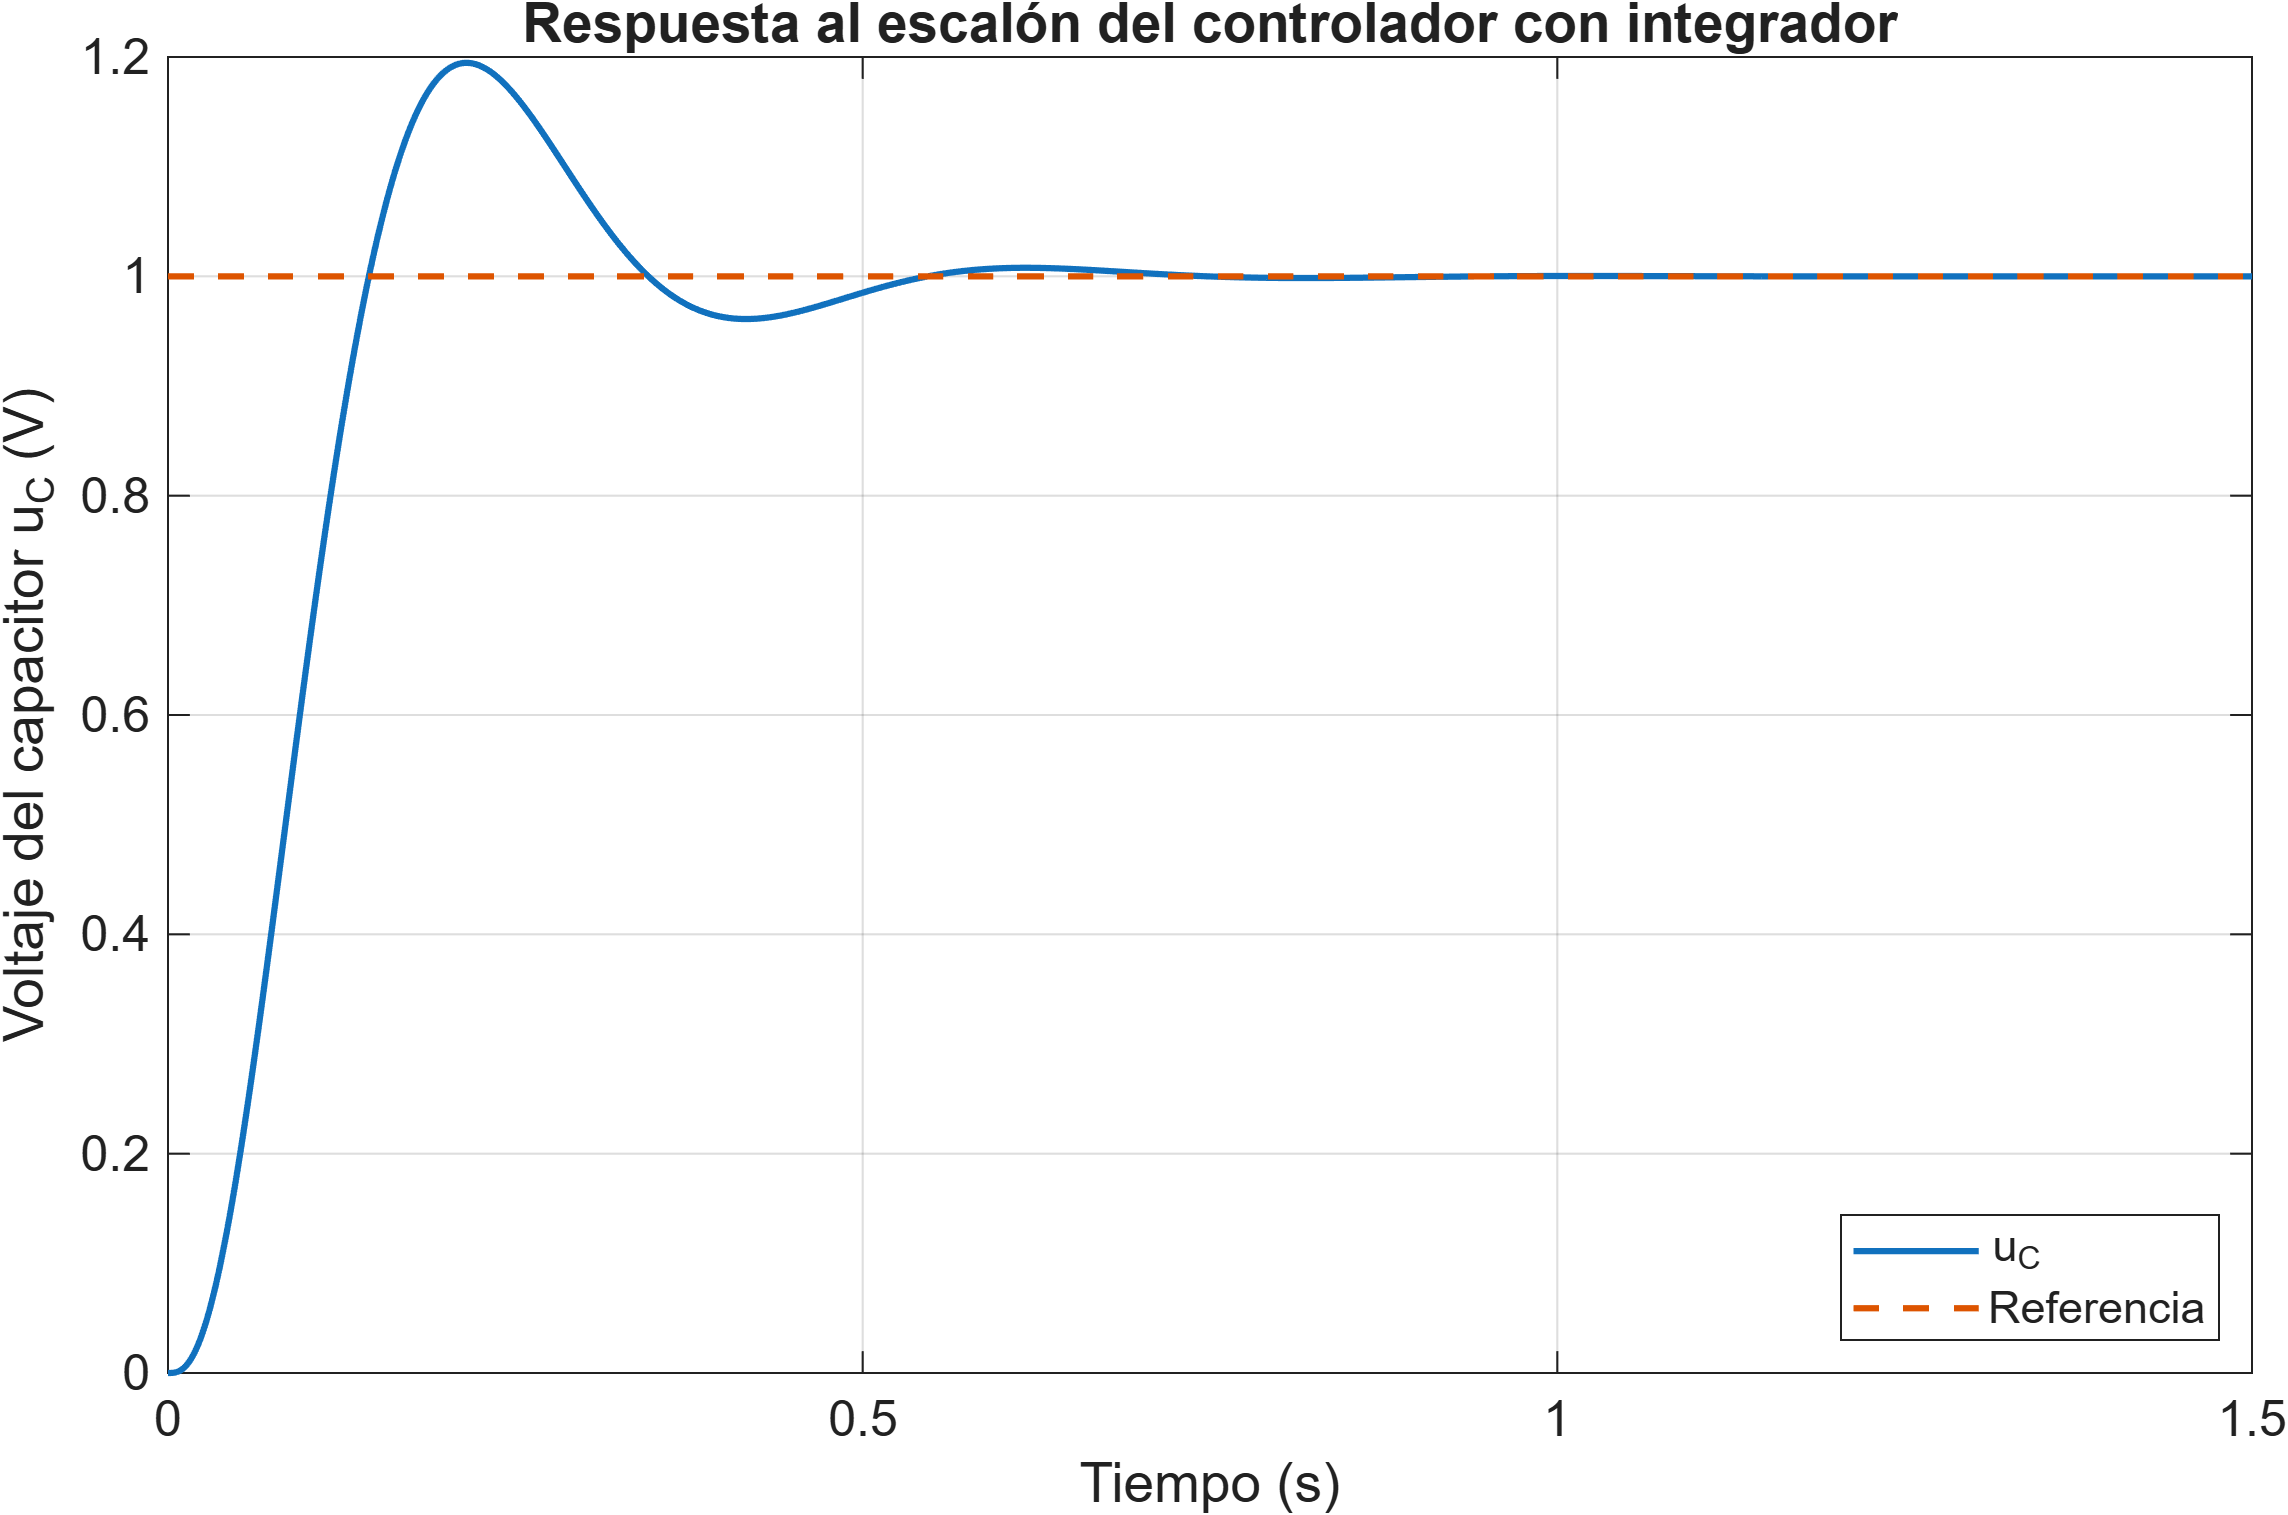
\includegraphics[width=\columnwidth]{escalon_controlador.png}
\caption{Respuesta al escalón del controlador con integrador.}
\label{fig:escalon}
\end{figure}

\subsection{Convergencia del observador}

La Fig.~\ref{fig:corriente} compara la corriente del inductor real con la estimada, obtenidas con \texttt{lsim} y las mismas condiciones iniciales que en Simulink. La corriente estimada arranca en 0.5\,A mientras que la real arranca en 0, y aproximadamente a los 0.06\,s ambas curvas coinciden. Esta figura es importante porque la corriente del inductor no se mide, así que el controlador depende completamente de su estimación.

\begin{figure}[!t]
\centering
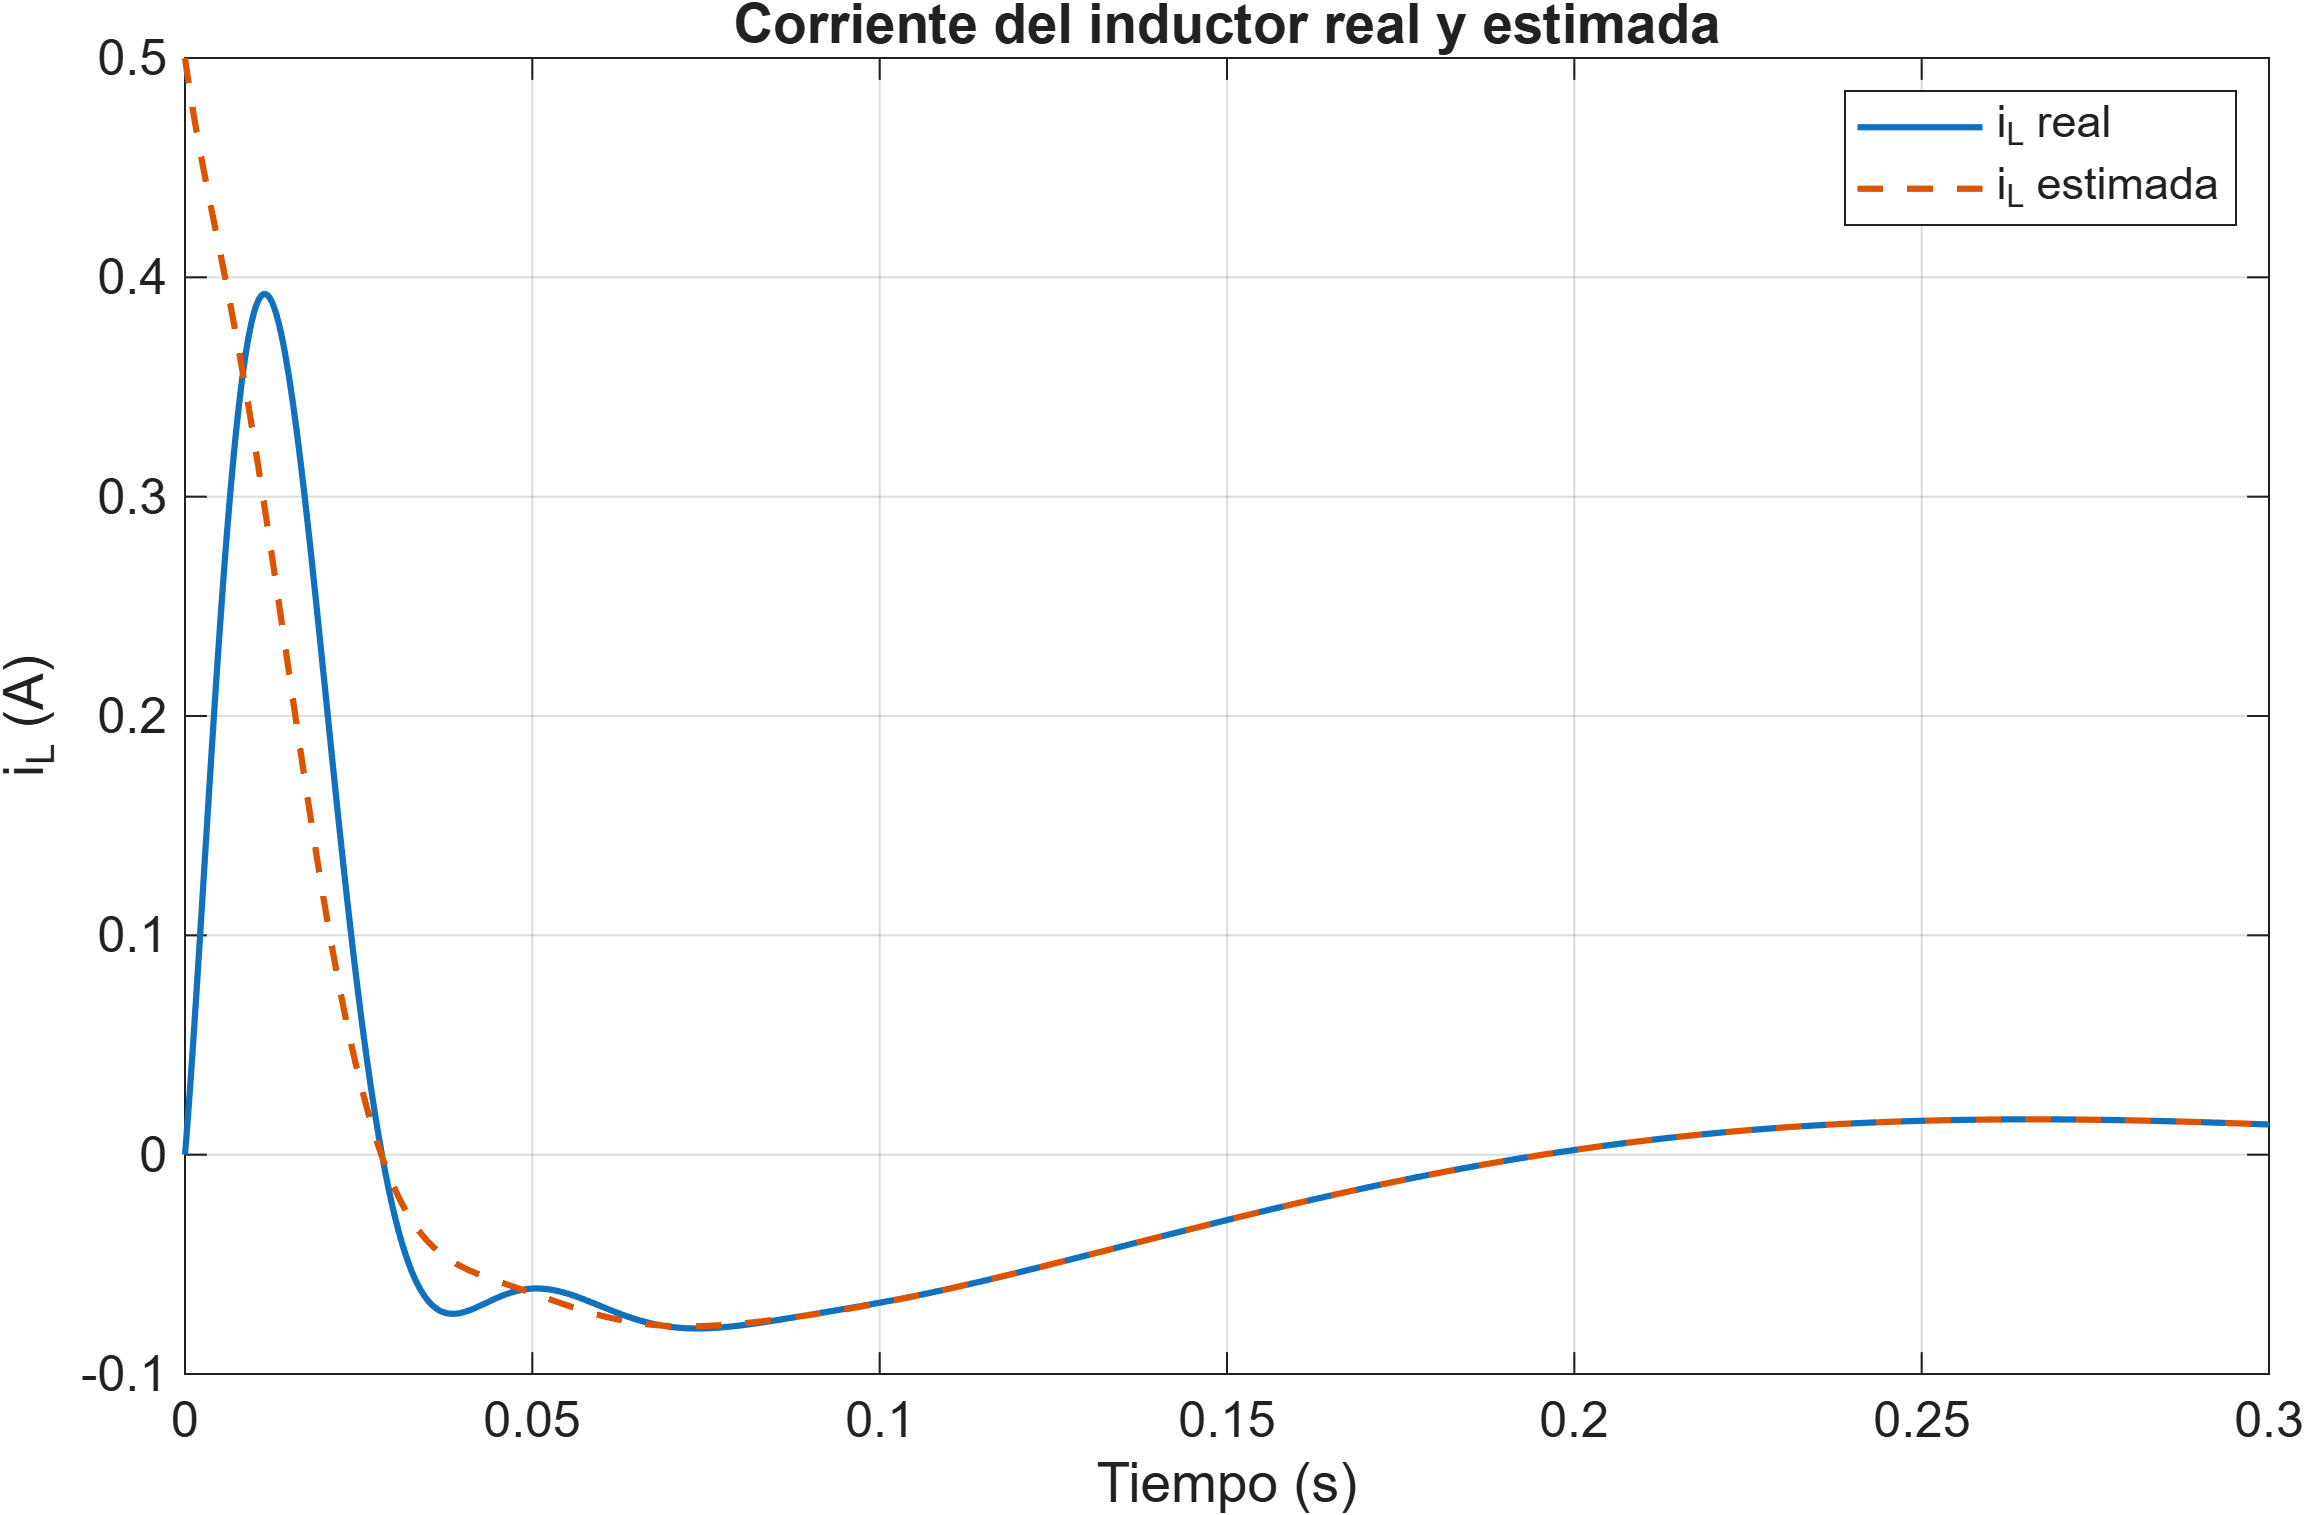
\includegraphics[width=\columnwidth]{corriente_estimada.png}
\caption{Corriente del inductor real y estimada con condiciones iniciales distintas.}
\label{fig:corriente}
\end{figure}

En Simulink, la Fig.~\ref{fig:obs_simulink} muestra el voltaje del capacitor real y el estimado, junto con el error de estimación. El estimado arranca en 1\,V y la planta en 0\,V; el error comienza en $-1$\,V y se hace prácticamente cero antes de 0.1\,s, lo que demuestra que el observador converge.

\begin{figure}[!t]
\centering
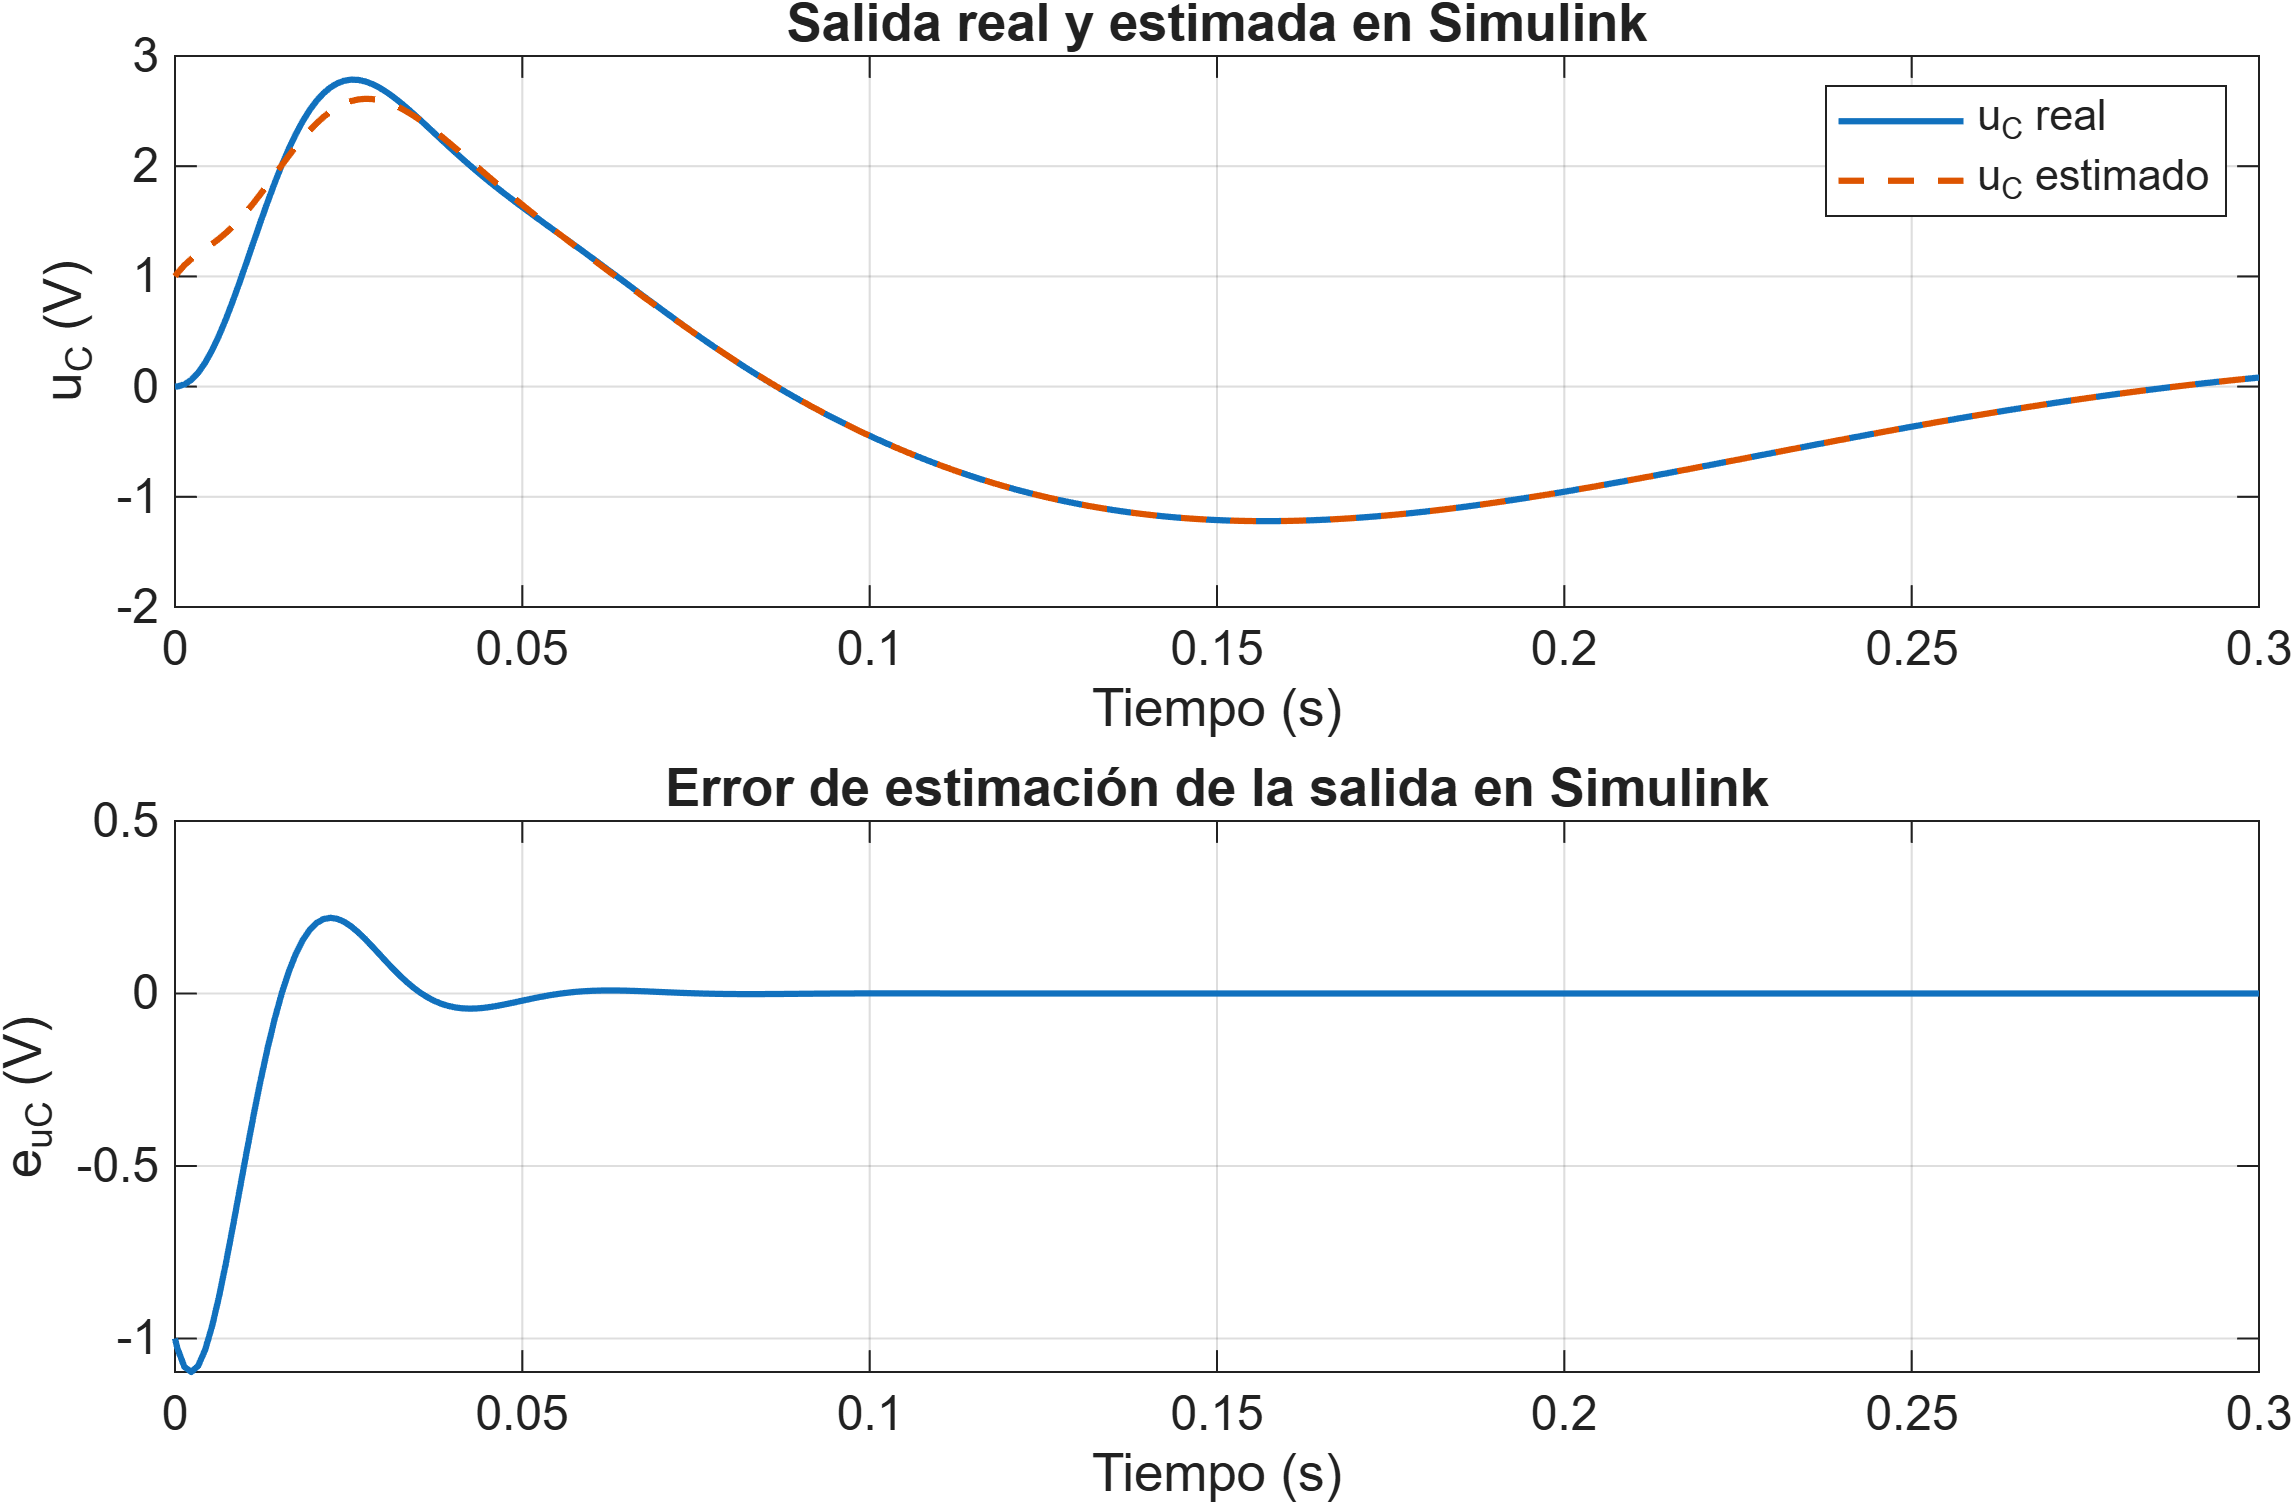
\includegraphics[width=\columnwidth]{observador_simulink.png}
\caption{Salida real y estimada, y error de estimación en Simulink.}
\label{fig:obs_simulink}
\end{figure}

\subsection{Sistema completo en Simulink}

La Fig.~\ref{fig:salida_simulink} muestra la salida del sistema completo. Durante el primer segundo aparece un transitorio causado por la diferencia de condiciones iniciales: mientras el observador converge, el controlador actúa con estados mal estimados y la salida llega a 2.8\,V y luego a $-1.2$\,V, pero vuelve a cero antes de que se aplique el escalón. Después de $t = 1$\,s la respuesta es igual a la de diseño: sobreimpulso cercano al 20\,\%, establecimiento en aproximadamente 0.5\,s y valor final de 1\,V. En estado estacionario la señal de control es de 0.5\,V, lo cual es coherente con la ganancia en DC de la planta, $83335/41665 = 2$.

\begin{figure}[!t]
\centering
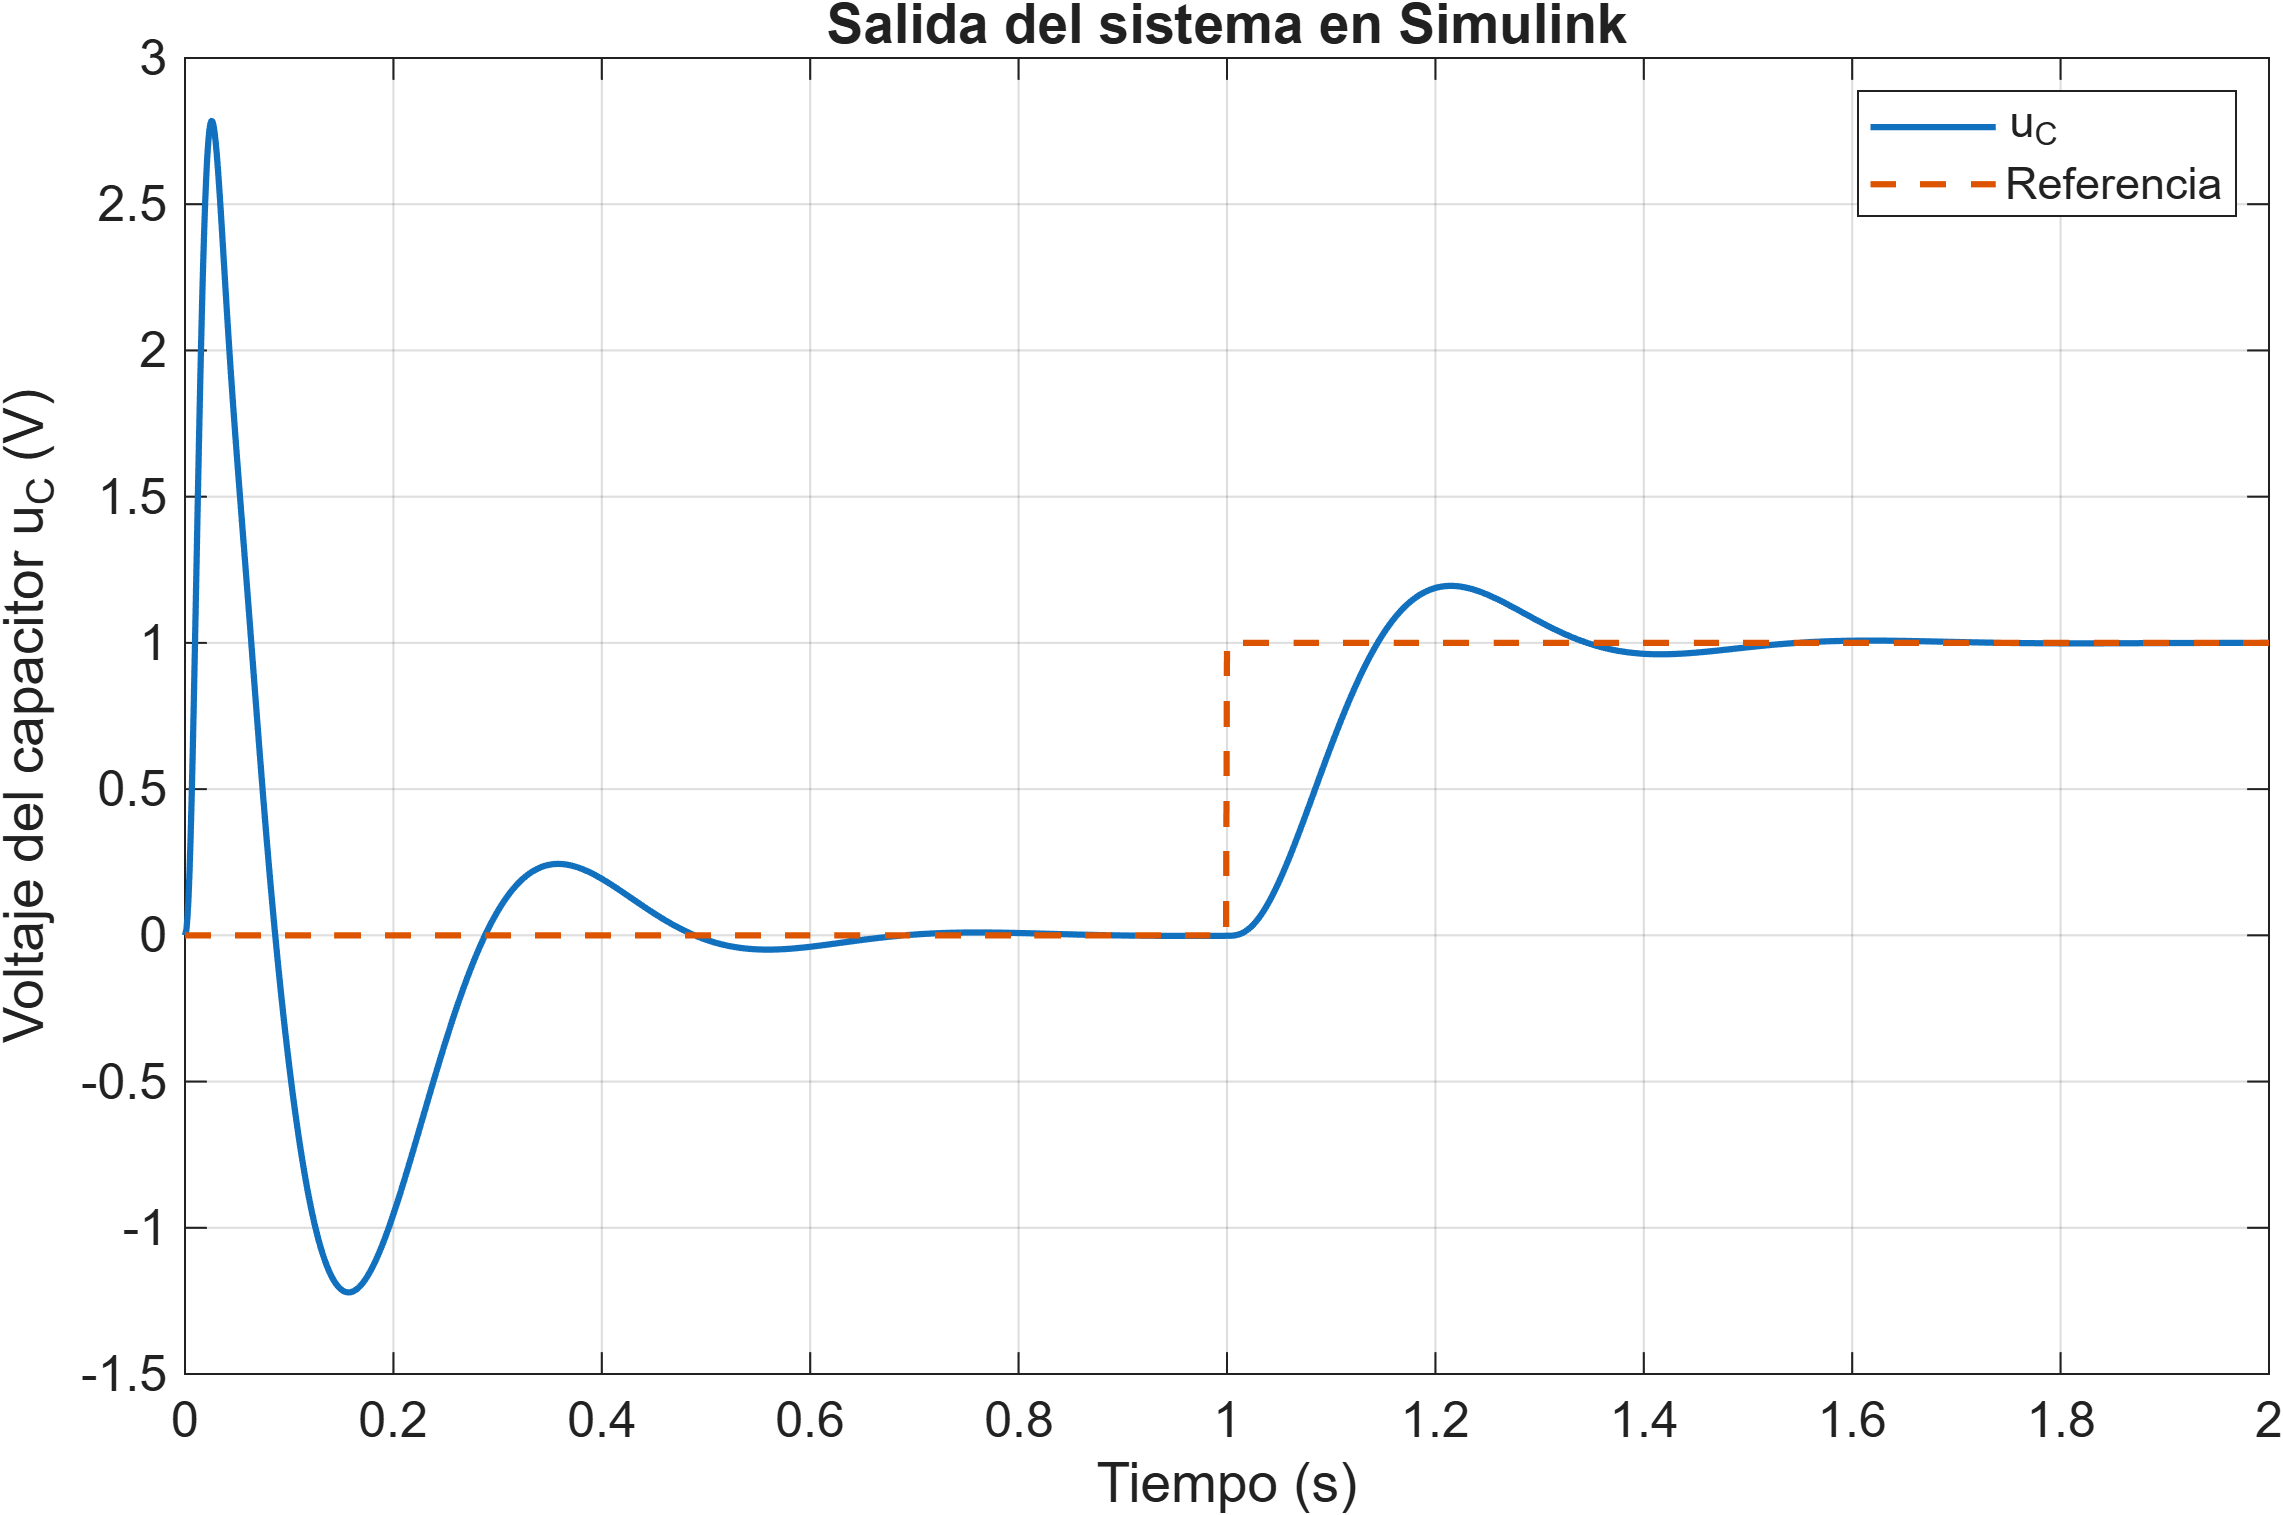
\includegraphics[width=\columnwidth]{salida_simulink.png}
\caption{Salida del sistema completo en Simulink.}
\label{fig:salida_simulink}
\end{figure}

\section{Conclusiones}

Se diseñó un controlador por realimentación de estados con acción integral y un observador para el convertidor DC-DC. El controlador cumple las especificaciones, con un sobreimpulso de 19.46\,\% y un tiempo de establecimiento de 0.487\,s, y el integrador elimina el error en estado estacionario.

El observador, con polos diez veces más rápidos que los del controlador, converge en menos de 0.1\,s aunque arranque con condiciones iniciales distintas a las de la planta. Esto se comprobó tanto en MATLAB como en Simulink. Los polos del sistema completo son la unión de los polos del controlador y los del observador, por lo que el observador no altera el diseño del controlador.

\pendiente{Conclusión sobre la respuesta de la IA y las dificultades encontradas.}

El transitorio inicial que aparece en Simulink muestra que, mientras el observador no ha convergido, el controlador actúa con información incorrecta. Por eso es conveniente que el observador sea bastante más rápido que el controlador.

\begin{thebibliography}{1}
\bibitem{nise}
N.~S. Nise, \emph{Control Systems Engineering}, 7th~ed. Hoboken, NJ, USA: Wiley, 2015.

\end{thebibliography}

\appendices
\section{Live Script de cálculos}
\label{ap:livescript}

\begin{lstlisting}
clear; clc; close all
format short g

%% Planta
Az = [0 -83.33 ; 500 -10]
Bz = [166.67 ; 0]
Cz = [0 1]
Dz = 0

[num, den] = ss2tf(Az,Bz,Cz,Dz);
G = tf(num, den)   % funcion de transferencia de la planta

%% Polos del controlador
M = 0.20      % sobreimpulso
ts = 0.5      % tiempo de establecimiento
xi = -log(M)/sqrt(pi^2+log(M)^2)
omegan = 4/(xi*ts)

syms s
ECC = s^2+2*xi*omegan*s+omegan^2;   % ecuacion caracteristica deseada del controlador
vpa(ECC, 6)
Rc = roots([1 2*xi*omegan omegan^2])   % polos del controlador

%% Observador
a1 = den(2);
a0 = den(3);
b0 = num(3);

% forma canonica observable
Ax = [-a1 1 ; -a0 0]
Bx = [0 ; b0]
Cx = [1 0]

Ox = [Cx ; Cx*Ax]   % matriz de observabilidad en forma canonica
Oz = [Cz ; Cz*Az]   % matriz de observabilidad del sistema original
rank(Oz)            % si es 2 el sistema es observable

% s^2 + (a1+l1)s + (a0+l2) = 0 ecuacion caracteristica del observador, se deben
% igualar los coeficientes a los de la ecuacion deseada para que el
% observador se comporte segun la ecuacion deseada

% polos 10 veces mas rapidos que el controlador
Ro = 10*Rc
ECOD = poly(Ro)               % ecuacion deseada del observador
vpa(poly2sym(ECOD, s), 6)

% igualando coeficientes
l1 = ECOD(2)-a1;
l2 = ECOD(3)-a0;
Lx = [l1 ; l2]   % ganancias del observador en forma canonica

P = inv(Oz)*Ox   % matriz de transformacion
Lz = P*Lx        % ganancias del observador en el sistema original

eig(Az-Lz*Cz)    % verificacion de los polos del observador

%% Controlador con integrador
syms k1 k2 ke
K = [k1 k2]
Aexp = [Az-Bz*K Bz*ke ; -Cz 0 ]   % matriz A expandida
Bexp = [0 ; 0 ; 1]
Cexp = [Cz 0]

ECA = collect(det(s*eye(3)-Aexp), s)   % ecuacion caracteristica del sistema expandido

p3 = 80;   % tercer polo
ECD = expand(ECC*(s+p3));   % ecuacion deseada del sistema expandido
vpa(ECD, 6)

% igualando coeficientes de ECA y ECD
cA = coeffs(ECA, s, 'All');
cD = coeffs(ECD, s, 'All');
sol = solve(cA(2:end) == cD(2:end), [k1 k2 ke]);
k1n = double(sol.k1)
k2n = double(sol.k2)
ken = double(sol.ke)

Kn = [k1n k2n]
Aen = [Az-Bz*Kn Bz*ken ; -Cz 0 ]
eig(Aen)   % verificacion de los polos del controlador

T = ss(Aen, Bexp, Cexp, 0);
stepinfo(T)   % sobreimpulso y tiempo de establecimiento obtenidos

%% Sistema completo
% estados: [x ; xN ; x estimado]
Alc = [Az Bz*ken -Bz*Kn ; -Cz 0 zeros(1,2) ; Lz*Cz Bz*ken Az-Bz*Kn-Lz*Cz ]
Blc = [0 ; 0 ; 1 ; 0 ; 0]
Clc = [Cz 0 0 0]

eig(Alc)   % polos del controlador y del observador

Tlc = ss(Alc, Blc, Clc, 0);
dcgain(Tlc)   % si da 1 no hay error de estado estacionario
\end{lstlisting}

\section{Respuesta íntegra de la IA}
\label{ap:ia}
\pendiente{Copiar aquí la respuesta completa de la IA al prompt de la Sección~IV.}

\end{document}
